\section{Solution}
    \subsection{Solution Overview}
        \begin{frame}
        \frametitle{Our Solution}
        \begin{itemize}
          \item Software As Apps
            \begin{itemize}
                \item Make tool size smaller by pushing generic functionality in the platform
            \end{itemize}
          \item Programs as Script
            \begin{itemize}
                \item Make tool components more like scripts, than programs, easier to customize
            \end{itemize}
          \item Platform and appstore
            \begin{itemize}
                \item Provide a platform and ecosystem to distribute these tools
            \end{itemize}

        %  deterministic \textbf{transformations} (\texttt{map}, \texttt{filter}, \texttt{join}, \ldots)
        %  \item \textbf{Actions} (\texttt{count}, \texttt{collect}, \texttt{reduce},
        %  \ldots) either return value or write to storage
        \end{itemize}
        \end{frame}

        \begin{frame}
            \frametitle{How to build Software as Apps?}
            \begin{figure}
                \centering
                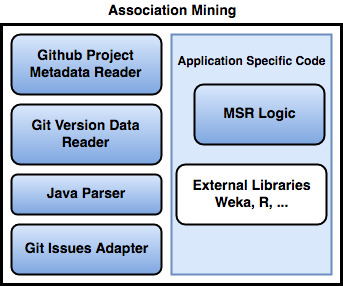
\includegraphics[scale=0.30]{figures/association.jpg}
                \caption{An MSR Tool Structure}
            \end{figure}
        \end{frame}

        \begin{frame}
            \frametitle{Pull supporting tools out and make them available as part of platform}
            \begin{figure}
                \centering
                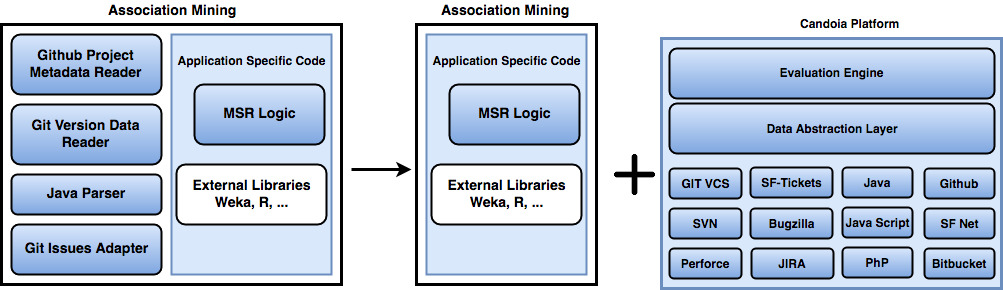
\includegraphics[width=0.75\linewidth]{figures/candoia_idea_overview.jpg}
                \caption{Repository Mining Tool Building}
            \end{figure}
        \end{frame}


        \begin{frame}
            \frametitle{How to build programs as Script?}
            \begin{figure}
                \centering
                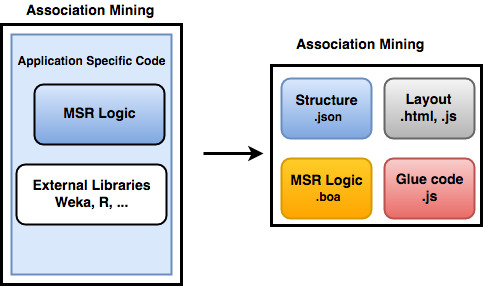
\includegraphics[scale=0.25]{figures/programtoscript.jpg}
                \caption{Transofrmation of MSR program to MSR tool}
            \end{figure}
        \end{frame}

        \begin{frame}
            \frametitle{MSR Tool as Candoia App}
            \begin{figure}
                \centering
                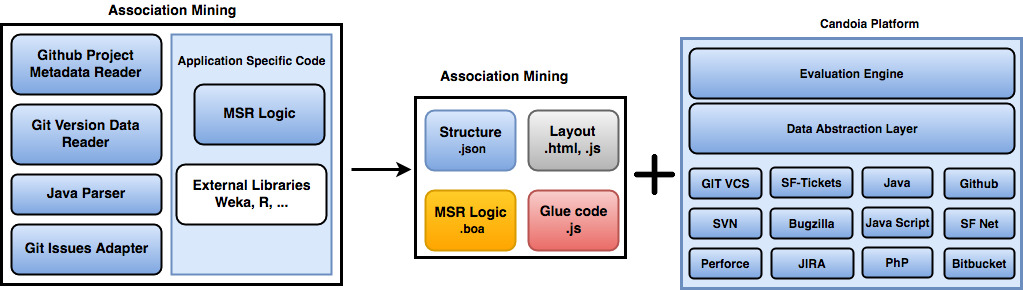
\includegraphics[width=0.75\linewidth]{figures/programstoscriptincandoia.jpg}
                \caption{MSR tool to Candoia App transformation}
            \end{figure}
        \end{frame}

        \begin{frame}
            \frametitle{Process Of Building and Sharing Candoia App}
            \begin{figure}
                \centering
                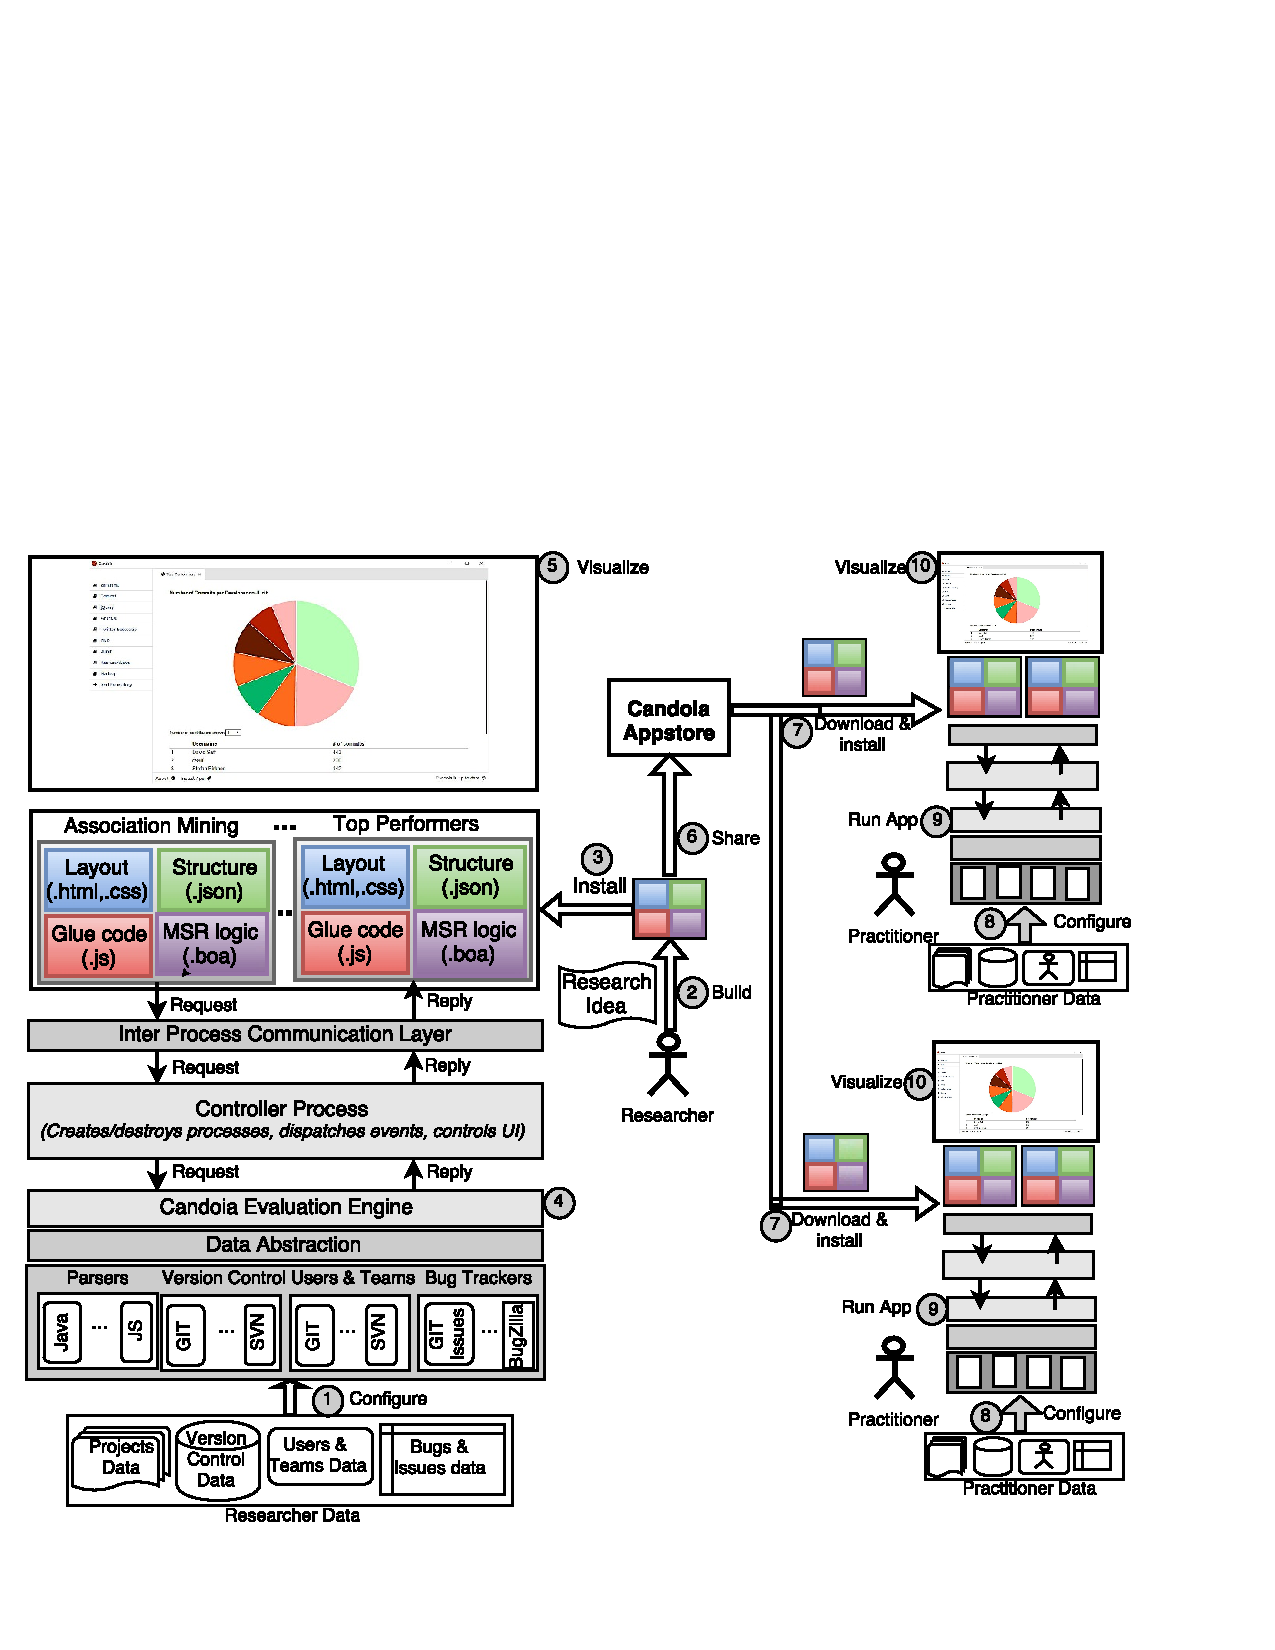
\includegraphics[width=0.6\linewidth]{figures/overview.pdf}
%                \caption{Repository Mining Tool Building}
            \end{figure}
        \end{frame}


    \subsection{Candoia Apps}
        \begin{frame}
        \frametitle{Candoia App Structure}
        \begin{columns}
            \column{0.45\textwidth}
                \begin{itemize}
                  \item Mining Logic
                    \begin{itemize}
                        \item Extension of Boa DSL
                    \end{itemize}
                  \item Visualization Layout
                    \begin{itemize}
                        \item Html
                        \item CSS
                    \end{itemize}
                  \item Glue Code
                    \begin{itemize}
                        \item Java script
                    \end{itemize}
                  \item Structure Decription
                    \begin{itemize}
                        \item Json %(file package.json)
                    \end{itemize}
                \end{itemize}

            \column{0.65\textwidth}
                \begin{figure}
                    \centering
                    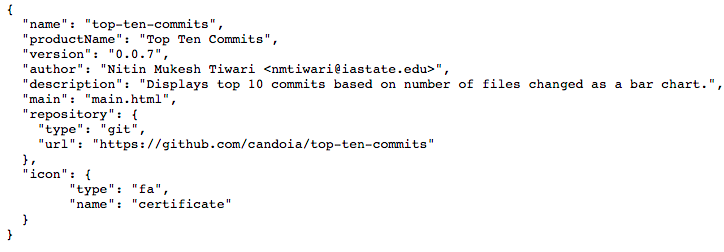
\includegraphics[scale=0.28]{figures/structure.png}
                    \caption{Structure of an Candoia app}
                \end{figure}
        \end{columns}
        \end{frame}

     \subsection{Data Abstraction}
        \begin{frame}
        \frametitle{Data Abstraction}
            \begin{itemize}
                \item Queries are written over data abstractions
               \item Data abstractions provide capability of running an app over data collected
               from diverse sources
               \item Candoia's data abstraction is extension of Boa DSL.
            \end{itemize}
        \end{frame}


    \subsection{Customization}
        \begin{frame}
        \frametitle{Customizations}
            Two levels of customizations
            \begin{itemize}
                \item Data source customizations
                \item App Customization
            \end{itemize}
        \end{frame}

        \begin{frame}
        \frametitle{Customizations}
            Two levels of customizations
            \begin{itemize}
                \item Data source customizations
                    \begin{itemize}
                        \item Concerned with changing the source of the data
                        \item No Change in app required
                        \item Just rerun the application with new datasource
                    \end{itemize}
                \item Customization in Apps
            \end{itemize}
        \end{frame}

        \begin{frame}
        \frametitle{Customizations}
            Two levels of customizations
            \begin{itemize}
                \item Data source customizations
                \item Customization in Apps
                    \begin{itemize}
                        \item Concerned with customizing different part of the apps
                        \item App customizations in Candoia are more focused in terms of findings the right component(s) for customizations
                    \end{itemize}
            \end{itemize}
        \end{frame}

        \begin{frame}
        \frametitle{Customizations}
            Two levels of customizations
            \begin{itemize}
                \item Data source customizations
                \item Customization in Apps
                    \begin{itemize}
                        \item Concerned with customizing different part of the apps
                        \item app customizations in Candoia are more focused in terms of findings the right component(s) for customizations
                        \end{itemize}
            \begin{figure}
                \centering
                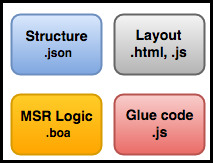
\includegraphics[scale=0.40]{figures/app.jpg}
                \caption{An MSR App Structure}
            \end{figure}
            \end{itemize}
        \end{frame}


        \begin{frame}
        \frametitle{Customizations}
            Two levels of customizations
            \begin{itemize}
                \item Data source customizations
                \item Customization in Apps
                    \begin{itemize}
                        \item Concerned with customizing different part of the apps
                        \item App customizations in Candoia are more focused in terms of findings the right component(s) for customizations
                        \item Script based app, easire to customize
                    \end{itemize}
            \end{itemize}
        \end{frame}


    \subsection{Evaluation Engine}
        \begin{frame}
            \frametitle{Candoia Evaluation Engine}
            \begin{itemize}
                \item Interpreter based Query evaluator for extended Boa DSL
            \end{itemize}
        \end{frame}

        \begin{frame}
            \frametitle{Candoia Evaluation Engine}
            \begin{itemize}
                \item Interpreter based Query evaluator of extended Boa DSL
                \item Reads data from local and remote software artifacts
                    \begin{itemize}
                        \item Forges: Github, Source Forge
                        \item VCS: GIT, SVN
                        \item Bug Tracker: Bugzilla, JIRA, Github-Issue, SF-Ticket
                        \item Programming Language: Java, Javascript
                    \end{itemize}
                \end{itemize}
            \end{frame}



        \begin{frame}
            \frametitle{Candoia Evaluation Engine}
            \begin{itemize}
                \item Interpreter based Query evaluator of extended Boa DSL
                \item Reads data from local and remote software artifacts
                    \begin{itemize}
                        \item Forges: Github, Source Forge
                        \item VCS: GIT, SVN
                        \item Bug Tracker: Bugzilla, JIRA, Github-Issue, SF-Ticket
                        \item Programming Language: Java, Javascript
                    \end{itemize}
                \item Process level parallelization for running multiple apps
                \item Thread level prarallelization for dataset creation
                \item Provides fine grained control to Candoia frontend
                \end{itemize}
            \end{frame}



    \subsection{Security Architecture}
        \begin{frame}
            \frametitle{Candoia Security Concern}
            \begin{itemize}
                \item Private software data
                    \begin{itemize}
                        \item Allow access to user data on a need to know basis
                    \end{itemize}
                \item Installing and running third party apps
                    \begin{itemize}
                        \item Prevent apps from corrupting each other
                        \item Prevent apps from accessing system resources directly
                    \end{itemize}
            \end{itemize}
         \end{frame}

        \begin{frame}
            \frametitle{Chromium based Candoia frontend}
            \begin{itemize}
                \item Candoia builds on the process architecture of Chromium, each window runs as a process
                \item Process communica tes with controller process via Inter Process Communication
                \item Controller process mediates interaction between file system, window data etc. by exposing APIs.
                \item An app can only access resources using exposed APIs.
            \end{itemize}
         \end{frame}
